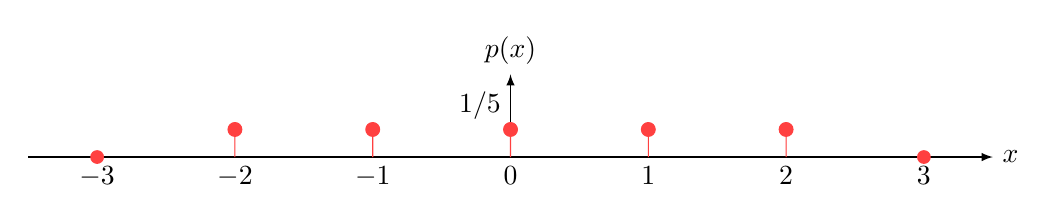
\begin{tikzpicture}[> = latex, scale=1.75]
    \def\r{0.05}
    % Axis
    \draw [->] (-3.5, 0) -- (3.5, 0) node [right] {$x$};
    \draw [->] (0, 0) -- (0, 0.6) node [above] {$p(x)$};
    \draw (0, 0.2) node [above left] {$1/5$};
    % Curve
    \foreach \x in {-2, -1, 0, 1, 2}{
        \draw (\x, 0) node [below] {$\x$};
        \draw [red!75, fill=red!75] (\x, 0) --++ (0, 0.2) circle (\r);
    }
    \fill [red!75] (-3, 0) circle (\r);
    \fill [red!75] (3, 0) circle (\r);
    \draw
        (-3, 0) node [below] {$-3$}
        (3, 0) node [below] {$3$};

\end{tikzpicture}